\section{Śledzenie promieni}

\subsection{Podstawowy algorytm śledzenia promieni}

Metoda śledzenia promieni pozwala określić widoczność obiektów znajdujących
się na scenie (a tym samym na generowanie obrazu) na zasadzie śledzenia umownych promieni świetlnych biegnących od obserwatora w scenę. W perspektywicznym rozumieniu sceny (a takiego dotyczy algorytm zaimplementowany na potrzeby tej pracy), pierwszym krokiem algorytmu jest wybranie środka rzutowania (nazywanego okiem obserwatora) oraz rzutni (powierzchnia na której zostanie odwzorowana trójwymiarowa scena). Rzutnię (a właściwie interesujący nas wycinek rzutni - abstrakcyjne okno obserwatora) można podzielić na regularną siatkę, w której każde pole odpowiada jednemu pikselowi ekranie urządzenia (tzw. układ urządzenia). Kolejnym krokiem algorytmu jest wypuszczenie promienia wychodzącego z oka obserwatora, przechodzącego przez dany piksel ekranu i lecącego dalej - w scenę. Kolor piksela jest ustalany na podstawie barwy i oświetlenia najbliższego obiektu (więcej o metodach oświetlenia można przeczytać w rozdziale !TU WSTAW ROZDZIAŁ!), który został przecięty przez wysłany promień. W przypadku braku kolizji piksel przybiera barwę otoczenia. 

\begin{center}
\adjustbox{valign=t}{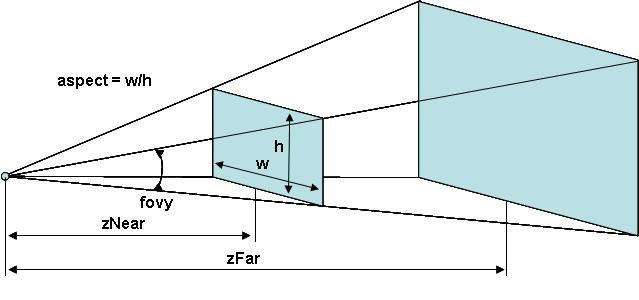
\includegraphics[width=10cm]{perspective_view.jpg}}
\end{center}

Poniżej przedstawiono pseudokod podstawowego śledzenia promieni

\begin{algorithmic}
\\
piksele, obiekty
\State obj = null
\State dist = max
\\
\State wybór środka rzutowania i rzutni
\\
\For{piksel in piksele}
	 \State wyznacz promień
	 \For{obiekt in obiekty}
	 \If {promień przecina obiekt i dystans $<$ dist}
    		\State obj = obiekt
    		\State dist = dystans
     \EndIf
	 \EndFor
\EndFor
\\
\State ustal kolor piksela na podstawie obj
\\
\end{algorithmic}


\subsection{Rekursywny algorytm śledzenia promieni}
\subsection{Równoległa wersja algorytmu śledzenia promieni}

\section{Wybór technologii}